\begin{fquestion}{Wie klassifiziert man Streuprozesse?}
    % Es gibt die 
    % \begin{itemize}
    %     \item elastische (keine Änderung der Teilchen),
    %     \item inelastische (Änderung der Teilchen oder Anregungen) und
    %     \item quasi-elastische (Nukleonen werden aus dem Kern gelöst)
    % \end{itemize}
    % Streuung.
    \emph{Elastische Streuung}: Die Energie des Projektils ist erhalten ($E' = E$ im Schwerpunktsystem), und es gibt keine Anregungen oder Umwandlungen des Target.
    
    \emph{Inelastische Streuung}: Die Energie des Projektils ist nicht erhalten ($E' \neq E$ im Schwerpunktsystem), und es kann Anregungen oder Umwandlungen des Target geben.
    
    \emph{Quasi-Elastische Streuung}: Grenzfall inelastischer Streuung für kleine Energieänderungen ($E' \approx E$ im Schwerpunktsystem).
\end{fquestion}

\begin{fquestion}{Welche Größen misst man zur Strukturauflösung?}
    Man misst die Energien und Impulse der Streuteilchen und Targetteilchen und damit einen winkelabhängigen Streuquerschnitt.
\end{fquestion}

\subsection{Elektronenstreuung an Wassermolekülen}

% Folgendes kann man damit auflösen:
% \begin{itemize}
%     \item Bindsungsenergien von H-Atomen in $\mathrm{H}_2 \mathrm{O}$,
%     \item mittlere Bindungsenergie der Nukleonen im O-Atom
% \end{itemize} 
% Siehe dazu Übung $\mathrm{H}_2 \mathrm{O}$-Spektrum, Streuspektrum, Zuordnung von Peaks und Effekten.

\begin{figure}[htb]
    \centering
    \includegraphics[width=0.5\linewidth]{img/povh_6_5.png}
    \caption{Energiespektrum von Elektronen, die an einem $\text{H}_2$O-Target gestreut wurden. 
    Die Daten wurden am Linearbeschleuniger MAMI-A in Mainz bei $\SI{246}{MeV}$ Strahlenergie unter einem Streuwinkel von $\SI{148.50}{\degree}$ aufgenommen.
    Deutlich erkennbar ist der Peak der elastischen Streuung an den quasi-freien Protonen in Wasserstoff bei $E' = \SI{160}{MeV}$. 
    Die Peaks rechts davon gehören zur elastischen Streuung am gesamten Sauerstoff-Kern. 
    Die breite Gauss-Verteilung entspricht der quasi-elastischen Streuung an Protonen im Sauerstoff-Kern. \refimgsourcebook{Povh}{Teilchen und Kerne}{978-3642378218}{85}}
    \label{fig:povh65}
\end{figure}
% 
% TODO: Figure 6.5 aus Povh, Particles and Nulcei, chapter 6.2.
% 
\begin{fquestion}{Welche Energie steht an der $x$-Achse?}
    Die Energie der gestreuten Elektronen, also $E' = \frac{E}{1 + \frac{E}{M}(1-\cos \theta)}$ (entspricht Compton-Streuung, Masse der Elektronen ist bei $E\sim \SI{100}{MeV}$ vernachlässigbar).
\end{fquestion}

\begin{fquestion}{Wo sieht man die initiale Energie der Elektronen?}
    Entspricht etwa der maximal gemessenen Energie eines gestreuten Elektrons, also ganz rechts auf der $x$-Achse.
    Üblicherweise ist $E \approx \SI{250}{MeV}$.
\end{fquestion}

\begin{fquestion}{Was für Peaks gibt es?}
    Die Bindungsenergien von H-Atomen in $\mathrm{H}_2 \mathrm{O}$ ist in der Größenordnung von eV, also gegenüber $E$ vernachlässigbar. 
    Die Elektronen streuen daher elastisch an den zugehörigen Protonen, und es gibt einen scharfen Peak bei der entsprechenden Energie $E'$. 
    Die Position ist abhängig von $\theta$ und $\frac{E}{M}$, wobei die Masse hier $M=m_p$.
    \\
    Es gibt einen weiteren scharfen, aber viel kleineren Peak für die Streuung am gesamten Sauerstoff-Kern. 
    Es ist $E_O' > E_H'$, da $M_O \approx 16m_p > m_p = M_H$.
    Der Peak liegt also deutlich weiter rechts.
    \\
    Zuletzt gibt es noch einen breiten Peak, der zur quasi-elastischen Streuung von Elektronen an Protonen im Sauerstoff-Kern gehört.
    Der Abstand des gauss-förmigen Peaks zum scharfen Peak des freien Wasserstoffs entspricht dabei gerade der Bindungsenergie $E_B$ der Protonen.
\end{fquestion}

\begin{fquestion}{Warum ist der quasi-elastische Peak so breit?}
    % Herauslösen von Protonen aus verschiedenen Energieniveaus im Kern ??? 
    Die relativ große Standardabweichung hängt mit dem großen Fermi-Impuls der Protonen über $\sigma_{\Delta E} = \frac{|\Vec{q}| p_F}{ M\sqrt{5}}$ zusammen.
    Insbesondere ist dafür die zufällige Richtung der Impulse relevant.
    Man kann $|\Vec{q}|$ über $E_\mathrm{elastisch}' = \frac{q^2}{2m_p}$ abschätzen, was gerade der Position des Wasserstoff-Peaks entspricht.
\end{fquestion}

\begin{fquestion}{Welchen interessanten Parameter des Kastenpotentials kann man dann abschätzen?}
    Aus dem Fermi-Impuls erhält man wie üblich auch die Fermi-Energie.
    Die Tiefe des Potentialkastens ist dann $V_0 = E_B + E_F$.
\end{fquestion}

% \begin{question}{Welche Energie muss dabei überwunden werden?}
%     Bindungsenergie zwischen den Nukleonen
% \end{question}

\begin{fquestion}{Wenn zwei Teilchen mit vergleichbarem Impuls elastisch stoßen, ist dann die Energie bei entgegengesetztem Impuls höher?}
    % Ja, weil größerer Relativ-Impuls und damit größerer $S$-Faktor ???
    Ja, weil der Relativ-Impuls dann größer ist, und dieser direkt in die Schwerpunktsenergie eingeht.
    Diese ist $\sqrt{s}$, wobei $s$ eine der drei Mandelstam-Variablen ist.
    Es gilt
    $$s = (p_1 + p_2)^2 = p_1^2 + p_2^2 + 2p_1\cdot p_2 = m_1^2 + m_2^2 + 2(E_1E_2 - \Vec{p}_1\cdot\Vec{p}_2).$$
    Damit wird also $\sqrt{s}$ für $\theta = \pi$ maximal.
\end{fquestion}

\subsection{Neutronenstreuung}

% \begin{question}{Warum Neutronen?}
%     elektrisch neutral, aber Spin aufgrund von Unterstruktur durch Quarks
% \end{question}

\begin{table}[H]
    \centering
    \begin{tabular}{|ll|ccc|}
        \hline
        Regime & Energie & & & \\
        \hline
        Kalt & $< \SI{1}{\milli\electronvolt}$ & \textcolor{red}{Beugung} & \textcolor{blue}{Elastisch} & \textcolor{Dandelion}{Einfang} \\
        Thermisch & $< \SI{0.5}{\electronvolt}$ & \textcolor{violet}{Kernspaltung} & \textcolor{blue}{Elastisch} & \textcolor{Dandelion}{Einfang} \\
        Epithermisch & $< \SI{50}{\kilo\electronvolt}$ & \textcolor{violet}{Kernspaltung} & \textcolor{blue}{Elastisch} & \textcolor{Dandelion}{Einfang} \\
        Schnell & $> \SI{50}{\kilo\electronvolt}$ & \textcolor{violet}{Kernspaltung} & \textcolor{blue}{Elastisch} & \textcolor{Dandelion}{Einfang} \\
        Medium & $> \SI{1}{\mega\electronvolt}$ &   & \textcolor{blue}{Elastisch} & \textcolor{Turquoise}{Inelastisch} \\
        Hochenergetisch & $> \SI{10}{\mega\electronvolt}$ &   & \textcolor{blue}{Elastisch} & \textcolor{Turquoise}{Inelastisch} \\
        \hline
    \end{tabular}
    \caption{Dominierende Wechselwirkungen (Beugung, Elastische Streuung sowie die nuklearen Reaktionen (Radioaktiver Einfang $(n, \gamma)$, andere Einfänge $(n, p)$ oder $(n, \alpha)$, Inelastische Streuung $(n, x)$ und Kernspaltung $(n, f)$) für Neutronen in verschiedenen Regimen.}
\end{table}

\begin{fquestion}{Was ist quasi-elastische Neutronenstreuung?}
    In der Festkörperphysik nutzt man die Methode der quasi-elastischen Neutronenstreuung (QENS), um Mittels kleiner Energieüberträge (unter $\si{\micro\electronvolt}$ Spektroskopie in der Größenordnung zwischen $1\ldots\SI{500}{\angstrom}$ zu studieren.
    
    Möglicherweise können im Rahmen der Teilchenphysik bei Energien um $6\ldots\SI{8}{MeV}$ die gebundenen Nukleonen beobachtet werden (Als Analogie zur quasi-elastischen Elektronenstreuung, Informationen sind hier schwer zu finden).
\end{fquestion}

\begin{fquestion}{Wie können Neutronen technisch erzeugt werden?}
    Abhängig vom gewünschten Energiebereich entweder durch Spallationsquellen (höhere Ausbeute für $E < \SI{0.1}{\mega\electronvolt}$ und $E>\SI{10}{\mega\electronvolt}$) oder Kernspaltung.
\end{fquestion}

\begin{fquestion}{Wie können Neutronen nachgewiesen werden?}
    Durch ${}^3\text{He}$- oder $\text{BF}_3$-Proportionalzählrohre mit der Reaktion ${}^3\text{He} + n \rightarrow {}^3\text{H} + p + \SI{0.764}{\mega\electronvolt}$.
    Alternativ mit Lithium-basierten Kristalldetektoren.
\end{fquestion}

\begin{fquestion}{Was ist der Vorteil von Neutronen für Streuprozesse?}
    Sie sind elektrisch neutral, können aber über ihr magnetisches Moment mit magnetischen und elektrischen Feldern wechselwirken.
    
    Außerdem ermöglicht die Dispersionsrelation der massiven Neutronen im Gegensatz zur steilen Dispersionsrelation von Photonen die Auflösung von kleinen Energien. 
\end{fquestion}

\begin{fquestion}{Wie sieht der Verlauf des Wirkungsquerschnitts von Neutronen aus?}
    Es ist $\dd \sigma \propto \frac{|p'|}{|p|} \dd \Omega$ mit den Impulsen $p$ vor und $p'$ nach der Streuung im Schwerpunktsystem.
    
    Für elastische Streuung ist $|p'| = |p|$ und entsprechend $\sigma = \mathrm{const.}$; für inelastische Streuung ist näherungsweise $|p'| = \mathrm{const.}$ (nach dem Einfang finden Kernprozesse statt, die wohldefiniert sind), entsprechend ist $\sigma \propto |p|^{-1} \propto E^{-1/2}$.
    
    \begin{center}
        \includegraphics[width=.8\linewidth]{img/Crosssection_Neutron.png}
    \end{center}
\end{fquestion}

% \begin{question}{Wofür verwendet man Neutronenstreuung noch?}
%     Anregung von Magnonen, hier Energie nur in Größenordnung von meV
% \end{question}

\begin{fquestion}{Warum braucht man thermische Neutronen zur Strukturauflösung in Festkörpern?}
    Aus der de-Broglie Gleichung ergibt sich 
    $$E_{\mathrm{kin}} = \frac{h^2}{2 m_{\mathrm{N}} \lambda^2} \approx \SI{20}{meV}$$
    für Neutronen mit einer Wellenlänge von $\SI{200}{pm}$, was in der Größenordnung von metallischen Gitterkonstanten $\approx \SI{400}{pm}$ liegt und damit durch Interferenz deren Struktur auflösen kann. 
\end{fquestion}


% \begin{question}{Was verwendet man üblicherweise?}
%     auch Neutronen
%     besser als Röntgenstrahlung, weil benachbare Elemente unterscheidbar, leichte Elemente auflösbar ???
%     Neutronen haben große freie Weglänge und sind zerstörungsfrei, also für große Proben geeignet
%     Effekte wie Antiferromagnetismus messbar ??? 
% \end{question}


\subsection{Rutherfordstreuung}

\begin{fquestion}{Was wollte Rutherford ursprünglich messen?}
    Rutherford untersuchte die Streuung von geladenen $\alpha$-Teilchen $\mathrm{He}^{2+}$ an Goldfolie.
    
    Zur Zeit des Experiments ging man vom Thompson'schen (bzw. Plum-Pudding) Atommodell aus, bei dem Elektronen und Protonen zusammen im Atomkern vermischt das Atom bilden.
    Dieses sollte durch den Streuversuch getestet werden.
    
    Tatsächlich stellte sich heraus, dass ein großer Teil der Projektile die Folie passierte und etwa jedes einhundertausendste reflektiert wurde, was mit dem Plum-Pudding Modell nicht zu erklären war.
\end{fquestion}

\begin{fquestion}{Wie sieht der Wirkungsquerschnitt aus?}
    Der Wirkungsquerschnitt bei Streuung an einer Punktladung unter der Coloumb-Wechselwirkung ist durch 
    $$\frac{\dd \sigma}{\dd \Omega} = \left( \frac{1}{4 \pi \varepsilon_0} \frac{Z_1 Z_2 e^2}{4 E_0}\right)^2 \frac{1}{\sin^4 \theta/2}$$
    gegeben. Hier sind $Z_1$ und $Z_2$ die Ladungszahlen der beiden Streupartner und $E_0$ die kinetische Energie des einfallenden Teilchens.
    Durch die Energieabhängigkeit ist $\sigma \propto E^{-2} \propto q^{-4}$.
    
    Bei höheren Auflösungen ist die Struktur des Kerns relevant, die zu einem zusätzlichen Faktor (dem Formfaktor) führt:
    $$\frac{\dd \sigma}{\dd \Omega}  = \left(\frac{\dd \sigma}{\dd \Omega} \right)_{\mathrm{Rutherford}} |F(q^2)|^2.$$
    
    Für eine homogen geladene Kugel mit Radius $R$ und Dichte $\rho_0$ ist in natürlichen Einheiten
    $$F(q^2) = \frac{4\pi \rho_0}{q^3} (\sin q R - q R \cos q R).$$
    Entsprechend lässt sich aus dem ersten Minimum die dimensionslose Größe $R q_{\mathrm{min}} = 2 R p \sin \theta/2 = 2 R E_0 \sin \theta/2$ ablesen. 
    Der Kernradius folgt dann aus dem Vergleich mit der ersten Nullstelle des Formfaktors bei $q R \approx 4.5$.

    \begin{center}
        Verlauf des Formfaktors einer homogen geladenen Kugel
        
        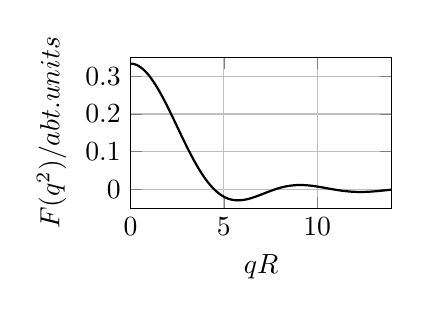
\begin{tikzpicture}
            \begin{axis}[
                xmin=0, xmax=14,
                ymin=-0.05, ymax=0.35, 
                xlabel={$qR$}, ylabel={$F(q^2) / \text{abt. units}$}, 
                % ytick distance = 0.5,
                grid=both]
                \addplot[domain = 1:14,smooth,samples=500, thick] {(sin(deg(x))- x * cos(deg(x))) / (x^3)};
                \addplot[domain = 0:1,smooth,samples=50, thick] {1/3 - x^2*4/5! + x^4*6/7! - x^6*8/9!};
            \end{axis}
        \end{tikzpicture}
    \end{center}    
\end{fquestion}

\begin{fquestion}{Was ist der Formfaktor $F(q^2)$?}
    Der Formfaktor
    $$F(q^2) = \int \rho(x) \e^{\i q x} \dd x$$
    ist die Fouriertransformierte der Ladungsverteilung.
    
    Dieser entsteht phänomenologisch aus folgender Überlegung: Vor und nach einem Streuprozess ist das Elektron ein freies Teilchen, entsprechend eine ebene Welle.
    Man macht den Ansatz einer ebenen einlaufenden und kugelförmigen auslaufenden Welle 
    $$\psi = \e^{ \i \vec{k} \cdot\vec{r} } + \frac{\e^{\i kr}}{r} f(\theta, \phi).$$
    Diese wird durch die Schrödingergleichung beschrieben, man findet 
    $$\frac{\dd \sigma}{\dd \Omega} = |f|^2.$$
    In der Born'schen Näherung ergibt sich dann schließlich die obige Form für Wirkungsquerschnitt und Strukturfaktor; intuitiv kann man sich das Auftreten der Minima also als destruktive Überlagerung verschiedener Streuungen vorstellen.
\end{fquestion}

% \begin{question}{Woher kommt die Form?}
%     mathematisch aus dem Formfaktor
%     anschaulich aus der Streuung von Neutronen an mehreren Nukleonen, also Interferenzen wie beim Doppelspalt ??? 
% \end{question}

% \begin{question}{Was ist der Formfaktor?}
%     FFT der Ladungsverteilung
% \end{question}

% \begin{question}{Wie bekommt man aus dem Wirkungsquerschnitt (harte, homogene Kugel) den Kernradius?}
%     das erste Minimum ist proportional zu $\frac{1}{R}$, Formfaktor ist $\frac{\sin (q)}{q}$ ??? 
% \end{question}

% \begin{question}{Was bedeutet das, wenn die Kugel sehr groß ist?}
%     Minimum verschiebt sich zu kleineren Winkeln
% \end{question}

\begin{fquestion}{Wie hängt der Wirkungsquerschnitt vom Kugelradius ab?}
    Das Produkt $q R \propto R \sin \frac{\theta}{2}$ ist für das erste Minima konstant.
    Entsprechend würde für größere Radien $R$ der Winkel $\theta$ kleiner und für kleinere Radien der Winkel $\theta$ größer werden.
    
    Anschaulich folgt dies aus der Unschärfe der Fouriertransformation.
    % \textcolor{red}{Anschaulich folgt dies aus der Unschärfe der Fouriertransformation.}
\end{fquestion}

% \begin{question}{Wie sieht das dann für das ursprüngliche Rutherford-Modell aus?}
%     Punktladung, $R$ gegen 0, also Minimum gegen unendlich, also Formfaktor konstant (mathematisch offensichtlich, da FFT von Dirac-Delta)
% \end{question}

\begin{fquestion}{Wie sieht die Ladungsdichteverteilung eines echten Kerns aus?}
    Bei großen Kernen ist die Näherung über eine homogene Ladungsdichte gerechtfertigt, in der Realität tritt noch ein diffuser Rand in der Ordnung $\SI{2.4}{fm}$ auf (zum Vergleich: $R = R_0 A^{1/3}$ mit $R_0 = \SI{1.25}{fm}$). 
    
    Bei kleineren Kernen (${}^4\mathrm{He}$, ${}^6\mathrm{Li}$ oder ${}^9\mathrm{Be}$) ist eine gauß-förmige Näherung eher gerechtfertigt, mit ebenfalls gauß-förmigem Formfaktor.
    
    Siehe \autoref{fig:ladungstraegerdichte formfaktor} für eine Visualisierung.
\end{fquestion}

\begin{fquestion}{Was ist der Mott-Formfaktor?}
    Beim Mott-Formfaktor 
    $$\left(\frac{\dd \sigma}{\dd \Omega}\right)_{\mathrm{Mott}} = \left(\frac{\dd \sigma}{\dd \Omega}\right)_{\mathrm{Rutherford}} (1 - \beta^2 \sin^2 \theta / 2) \xrightarrow[\beta = 1]{} \left(\frac{\dd \sigma}{\dd \Omega}\right)_{\mathrm{Rutherford}} \cos^2 \theta / 2 $$
    wird zusätzlich der Spin des Elektrons berücksichtigt.
    
    Für hohe Energien muss man ebenfalls den Targetrückstoß berücksichtigen, durch welchen ein zusätzlicher Faktor
    $$\left(\frac{\dd \sigma}{\dd \Omega}\right)_{\mathrm{Mott}} = \left(\frac{\dd \sigma}{\dd \Omega}\right)_{\mathrm{Mott}}^* \frac{E'}{E}$$
    durch ein sich änderndes Phasenraumvolumen eingeführt wird.
\end{fquestion}

% \begin{question}{Wie sieht das bei größeren Kernen aus?}
%     Radius wird größer, aber Ladungsdichte bleibt gleich
% \end{question}

% \begin{question}{Wie kann man das Auftreten der Minima erklären?}
%     Elektron streut als eben Welle am kern, Überlagerung der gestreuten Wellenfronten von verschiedenen Stellen des Kerns erzeugt destruktive Interferenz
% \end{question}

\subsection{Elektronenstreuung am Kern}

\begin{table}[H]
    \centering
    \begin{tabular}{m{4cm}>{\centering}m{3cm}>{\centering}m{3cm}m{4cm}}
        & $\rho(r)$ & $F(q^2)$ & \\
        $\rho(r) = \frac{\delta(r)}{4\pi}$ & 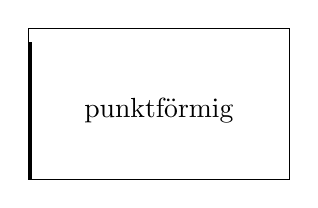
\begin{tikzpicture}
\pgfplotsset{%
    width=4.9cm,
    height=3.5cm
}
            \begin{axis}[domain=0:1, xmin=0, xmax=1, ymin=0, ymax=1.1, ticks = none]
                \draw[-, line width=1mm, black] (axis cs:0,0) -- (axis cs:0,1);
                \node[] at (axis cs: .5,.5) {\normalsize
 punktförmig};
            \end{axis}
        \end{tikzpicture}
 & 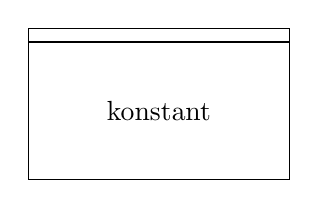
\begin{tikzpicture}
\pgfplotsset{%
    width=4.9cm,
    height=3.5cm
}
            \begin{axis}[domain=0:1, xmin=0, xmax=1, ymin=0, ymax=1.1, ticks = none]
                \addplot [thick, black, samples=50] {1};
                \node[] at (axis cs: .5,.5) {\normalsize
 konstant};
            \end{axis}
        \end{tikzpicture} & $F(q^2)=1$ \\
    $\rho(r) = \frac{a^3}{8\pi} e^{-a r}$ &  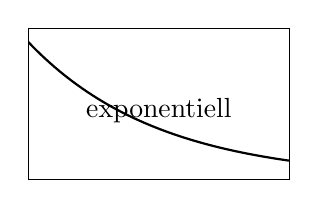
\begin{tikzpicture}
\pgfplotsset{%
    width=4.9cm,
    height=3.5cm
}
            \begin{axis}[domain=0:1, xmin=0, xmax=1, ymin=0, ymax=1.1, ticks = none]
                \addplot [thick, black, samples=50] {exp(-2*x)};
                \node[] at (axis cs: .5,.5) {\normalsize
 exponentiell};
            \end{axis}
        \end{tikzpicture} &  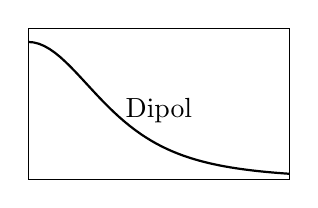
\begin{tikzpicture}
\pgfplotsset{%
    width=4.9cm,
    height=3.5cm
}
            \begin{axis}[domain=0:1, xmin=0, xmax=1, ymin=0, ymax=1.1, ticks = none]
                \addplot [thick, black, samples=50] {(1 + 4 * x^2)^(-2)};
                \node[] at (axis cs: .5,.5) {\normalsize
 Dipol};
            \end{axis}
        \end{tikzpicture} & $F(q^2) = \left(1 + \frac{q^2}{a^2 \hbar^2}\right)^{-2}$ \\
    $\rho(r) = \sqrt[3]{\frac{a^2}{2\pi}} e^{-\frac{a^2 r^2}{2}}$ & 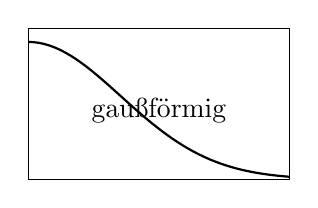
\begin{tikzpicture}
\pgfplotsset{%
    width=4.9cm,
    height=3.5cm
}
            \begin{axis}[domain=0:1, xmin=0, xmax=1, ymin=0, ymax=1.1, ticks = none]
                \addplot [thick, black, samples=50] {exp(-4*x^2)};
                \node[] at (axis cs: .5,.5) {\normalsize
 gaußförmig};
            \end{axis}
        \end{tikzpicture} & 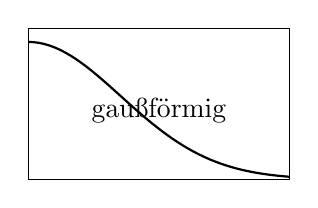
\begin{tikzpicture}
\pgfplotsset{%
    width=4.9cm,
    height=3.5cm
}
            \begin{axis}[domain=0:1, xmin=0, xmax=1, ymin=0, ymax=1.1, ticks = none]
                \addplot [thick, black, samples=50] {exp(-4*x^2)};
                \node[] at (axis cs: .5,.5) {\normalsize
 gaußförmig};
            \end{axis}
        \end{tikzpicture} & $F(q^2) = e^{-\frac{q^2}{2 a^2 \hbar^2}}$ \\
    $\rho(r) = \begin{cases} \frac{3}{4 \pi R^3} & r\leq R \\ 0 & r > R \end{cases}$ & \begin{tikzpicture}
\pgfplotsset{%
    width=4.9cm,
    height=3.5cm
}
            \begin{axis}[domain=0:1, xmin=0, xmax=1, ymin=0, ymax=1.1, ticks = none]
                \addplot [thick, black, samples=100] {1/(1+exp((x-0.5)/0.00001))};
                \node[] at (axis cs: .5,.5) {\normalsize
 Homogene Kugel};
            \end{axis}
        \end{tikzpicture} & 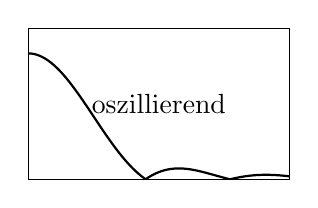
\begin{tikzpicture}
\pgfplotsset{%
    width=4.9cm,
    height=3.5cm
}
            \begin{axis}[domain=0:10, xmin=0, xmax=10, ymin=0, ymax=0.4, ticks = none]
                \addplot[domain = 1:10,smooth,samples=500, thick] {abs((sin(deg(x))- x * cos(deg(x))) / (x^3))};
                \addplot[domain = 0:1,smooth,samples=50, thick] {1/3 - x^2*4/5! + x^4*6/7! - x^6*8/9!};
                \node[] at (axis cs: 5,.2) {\normalsize
 oszillierend};
            \end{axis}
        \end{tikzpicture} & $F(q^2) = \frac{3(\sin x - x \cos x)}{x^3}$, wobei $x = |q|R / \hbar$\\
    $\rho(r) = \frac{\rho_0}{1 + e^{\frac{r - c}{a}}}$ & 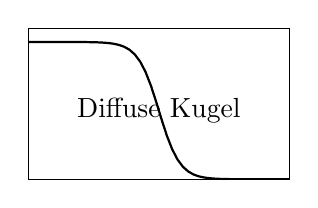
\begin{tikzpicture}
\pgfplotsset{%
    width=4.9cm,
    height=3.5cm
}
            \begin{axis}[domain=0:1, xmin=0, xmax=1, ymin=0, ymax=1.1, ticks = none]
                \addplot [thick, black, samples=50] {1/(1+exp((x-0.5)/0.04))};
                \node[] at (axis cs: .5,.5) {Diffuse Kugel};
            \end{axis}
        \end{tikzpicture} & 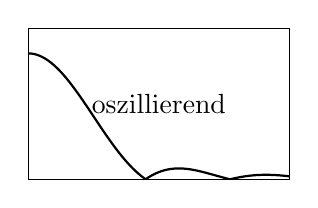
\begin{tikzpicture}
\pgfplotsset{%
    width=4.9cm,
    height=3.5cm
}
            \begin{axis}[domain=0:10, xmin=0, xmax=10, ymin=0, ymax=0.4, ticks = none]
                \addplot[domain = 1:10,smooth,samples=500, thick] {abs((sin(deg(x))- x * cos(deg(x))) / (x^3))};
                \addplot[domain = 0:1,smooth,samples=50, thick] {1/3 - x^2*4/5! + x^4*6/7! - x^6*8/9!};
                \node[] at (axis cs: 5,.2) {\normalsize
 oszillierend};
            \end{axis}
        \end{tikzpicture} & Keine analytische Form
        \\
        & $r \rightarrow \infty$ & $q \rightarrow \infty$ &
    \end{tabular}
    \caption{Gegenüberstellung verschiedener Ladungsträgerdichten $\rho(r)$ und ihrer Formfaktoren $F(q^2)$.}
    \label{fig:ladungstraegerdichte formfaktor}
\end{table}

% (Streuquerschnitt für eine diffuse Kugel)

% \begin{question}{Wo sieht man den Kernabstand?}
%     Das erste Minimum des Formfaktors $F(q^2)$ ist proportional zu $\frac{1}{r_0}$.
% \end{question}

% \begin{question}{Kann bei Auflösung mehrerer Teilchen mehr Energie haben, als bei einem einzelnen?}
%     nein, die Streuung an einem Teilchen (z.B. Punktladung) gibt Maxima
%     die Streuung an vielen Nukleonen bringt durch Überlagerung nur (kleinere) Nebenmaxima und zusätzliche Minima (vergleiche Interferenzmuster von $N$ Spalten in Optik).
% \end{question}

\begin{fquestion}{Was passiert bei der Elektron-Kern-Streuung bei höheren Energien?}
    Nach den elastischen Stoßprozessen kommen zunächst die \textit{inelastischen Kernanregungen}, dort werden bei einigen $\SI{10}{MeV}$ Riesendipolresonanzen und Übergänge zwischen Kernzuständen angeregt.
    
    Danach finden elastische Stoßprozesse an den einzelnen Nukleonen bei Energien von $\SI{0.2}{GeV}\ldots\SI{10}{GeV}$ statt, durch welche die elektrischen und magnetischen Eigenschaften von Proton und Neutron untersucht werden können. 
    Man beobachtet, dass das Proton einen Dipolformfaktor entsprechend einer exponentiellen Ladungsverteilung aufweist.
    
    In diesem Energiebereich kann man bei größeren Kernen (Beispiel: $\text{H}_2$O) über \textit{quasi-elastische Streuung} (Wechselwirkung mit nur einem Nukleon im Kern, welches danach aus dem Verband gelöst ist) die Tiefe des Kernpotentials ($17\ldots\SI{44}{MeV}$, aus der Verschiebung zur elastischen Streuung) sowie den Fermi-Impuls ($170 \ldots \SI{270}{MeV/c}$, aus der Breite der Verteilung) bestimmen.
    
    Bei noch größeren Energie von einigen $\SI{100}{GeV}$ kommt es zu \textit{tiefinelatischen Stößen}, bei denen die Unterstruktur (Quarks) der Nukleonen aufgelöst werden können.
    Hier beobachtet man beispielsweise die $\Delta^+$-Resonanz des Protons bei einer Masse von $W=\SI{1232}{MeV}$ ($|\Delta^+\rangle = |\mathrm{u}^\uparrow \mathrm{u}^\uparrow \mathrm{d}^\uparrow \rangle$, siehe auch Povh, 16.2 Baryonenmultipletts).
    
    Misst man die Strukturfunktionen, kann man außerdem bestimmen dass der Wirkungsquerschnitt unabhängig von $q^2$ ist, man also an punktförmigen Teilchen streut und die Konstituenten des Protons den Spin $1/2$ tragen müssen.
\end{fquestion}

% \begin{question}{Was passiert bei noch höheren Elektronenergien?}

%     Man kann die Ladungsverteilung der Protonen im Kern auflösen.
%     Anhand der gemessenen Formfaktoren kann man auf die Struktur des Nukleons schließen.
%     % Formfaktoren, kann aus Streubildern auf die Verteilung des Streutargets schließen
% \end{question}

% \begin{question}{Was passiert bei noch höheren Energien?}
%     Auflösung der Quark-Struktur der Protonen bzw. Quarkanregungen (bspw. $\Delta^+$-Resonanz, also $|\mathrm{u}_\uparrow \mathrm{u}_\uparrow \mathrm{d}_\uparrow \rangle$ mit Spin 3/2.)
% \end{question}

\begin{fquestion}{Welche Anregungen kann man bei Quarks beobachten?}
    Bei Quarks wurden bisher keine Anregungen gefunden, weshalb man davon ausgeht, dass es sich um fundamentale Teilchen ohne Unterstruktur handelt.
    
    Bei Nukleonen kann man hingegen Spin-Anregungen wie die Delta-Resonanzen beobachten.
    Möglich sind auch Anregungen im Kern.
\end{fquestion}

\begin{fquestion}{Wie viele Größen braucht man, um Streuung zu beschreiben?}
    Für die elastische Streuung benötigt man einen Parameter (etwa den Streuwinkel $\theta$).
    
    Bei der inelastischen Streuung benötigt man zusätzlich einen weiteren Parameter, beliebte Paare sind etwa $(E', \theta)$, $(q^2, \nu)$ oder $(q^2, x)$.
    Hier ist 
    $$\nu \equiv \frac{Pq}{M} \xrightarrow[\text{Labor}]{} E - E'$$
    ein Maß für den Energieübertrag und die Bjorken'sche Skalenvariable
    $$x = \frac{q^2}{2 M \nu}$$
    ein Maß für die Inelastizität des Prozesses.
    Bei $x=1$ ist der Prozess vollkommen elastisch, für $0 < x < 1$ entsprechend inelastisch.
\end{fquestion}

\begin{fquestion}{Was ist die anschauliche Bedeutung der Bjorken'schen Skalenvariable bei hohen Energien?}
    In der Stoßnäherung (quasi-elastisch: Wechselwirkung mit den individuellen Partonen) gibt $x$ den Anteil eines einzelnen Partons (bei vernachlässigbarer Ruhemasse) am Gesamtimpuls des Nukleons an.
\end{fquestion}